\section{Propiedades de $\mathbb{R}$}

$(\mathbb{R}, +,\cdot)$ es un campo. 


\begin{definicion}
	Un conjunto no vacío $P$ de elementos de un campo $\mathbb{F}$ es una clase positiva si cumple: 
	\begin{enumerate}
		\item Si $a,b\in P\implies a+b\in P$.
		\item Si $a,b\in P\implies a\cdot b\in P$. 
		\item Si $a\in\mathbb{F}$, entonces: 
		\begin{enumerate}
			\item $a\in P$ o  $a=0$ o $-a\in P$. (Ley de tricotomía) 
		\end{enumerate}
	\end{enumerate}
\end{definicion}

\begin{nota}
	Sea $N=\{-a:a\in P\}$ la clase negativa relativa a $P$. $\implies\mathbb{F}=P\cup \{0\}\cup \mathbb{N}$.
\end{nota}

\begin{ejemplo}
	\begin{enumerate}
		\item $(\mathbb{Q},+,\cdot)$ es un campo. Sea $P\{a/b\in \mathbb{Q}\ni a,b\in\mathbb{Z}^+\}\implies P$ es una clase positiva de $\mathbb{Q}$. 
		\item Sea $\mathbb{Z}_2=\{0,1\}$, en las operaciones: 

	\begin{table}[h]
		\centering
		\begin{tabular}{@{}|c|c|c|@{}}
			\toprule
			+ & 0                        & 1                        \\ \midrule
			0                         & {\color[HTML]{FE0000} 0} & {\color[HTML]{FE0000} 1} \\ \midrule
			1                         & {\color[HTML]{FE0000} 1} & {\color[HTML]{FE0000} 0} \\ \bottomrule
		\end{tabular}
	\end{table}

	\begin{table}[h]
		\centering
		\begin{tabular}{@{}|c|c|c|@{}}
			\toprule
			* & 0                        & 1                        \\ \midrule
			0                         & {\color[HTML]{FE0000} 0} & {\color[HTML]{FE0000} 0} \\ \midrule
			1                         & {\color[HTML]{FE0000} 0} & {\color[HTML]{FE0000} 1} \\ \bottomrule
		\end{tabular}
	\end{table}	
$\implies(\mathbb{Z}_2,+,\cdot)$ es un campo. 
\begin{enumerate}
	\item Sea $P=\{0\}$. Cumple las propiedades: 1, 2. No cumple 3. $\implies P$ no es una clase positiva de $\mathbb{Z}_2$.
	\item Sea $P'=\{1\}$. No cumple el 1. $\implies P'$ no es clase positiva de $\mathbb{Z}_2$.   
\end{enumerate}
	\end{enumerate}
\end{ejemplo}

\begin{definicion}
	Sea $P$ la clase positiva del campo $\mathbb{F}$, entonces se dice que $\mathbb{F}$ está ordenada por $P$ (o que $\mathbb{F}$ es un campo ordenado).
	\begin{enumerate}
		\item Si $a\in P$, se dice que $a$ es positivo. Notación $a>0$. 
		\item Si $a\in P$ o $a=0$, se dice que $a$ es no negativo. Notación $a\geq 0$. 
		\item Si $a,b\in \mathbb{F}$ y $a-b\in P$, se escribe $a>b$. 
		\item Si $a,b\in\mathbb{F}$ y $a-b\in P$ o $a-b=0$, se escribe $a\geq b$.
	\end{enumerate}
\end{definicion}

\begin{prop} Otras propiedades:
	\begin{enumerate}
		\item Si $a>b$ y $b>c\implies a>c$. 
		\item Si $a,b\in \mathbb{F}$, entonces 
		\begin{enumerate}
			\item $a>b$ o $a=b$ o $b>a$. 
		\end{enumerate}
	\item Si $a\geq b$ y $b\geq a\implies a=b$.
	\end{enumerate}
\end{prop}

\begin{prop}
	Sea $\mathbb{F}$ un campo ordenado:
	\begin{enumerate}
	\item Si $a\neq 0\implies a^2>0$. 
	\item 1>0. 
	\item Si $n\in \mathbb{Z}^+\implies n>0$. 	
	\end{enumerate}
\end{prop}

\begin{teorema}
	Sean $a,b,c\in \mathbb{F}$. 
	\begin{enumerate}
		\item Si $a>b\implies a+c>b+c$.
		\item Si $a>b$ y $c>d\implies a+c>b+d$.
		\item Si $a>b$ y $c>0\implies ac>bc$. 
		\item Si $a>b$ y $c<0\implies ac<bc$.
		\item Si $a>0\implies a^{-1}>0$. 
		\item Si $a<0\implies a^{-1}<0$.  
	\end{enumerate}
\end{teorema}

\begin{corolario}
	Si $a>b\implies a>\frac{a+b}{2}>b$. 
	\begin{nota}
		Hagamos $b=0$. Entonces, si $a>0\implies a>\frac{a}{2}>0$. Entonces, en un campo ordenado no existe un número positivo menor. 
	\end{nota}
\end{corolario}

\begin{teorema}
	Si $ab>0$, entonces, $a>0$ y $b>0$ o $a<0$ y $b<0$. 
\end{teorema}

\begin{definicion}
	Sea $\mathbb{F}$ un campo una clase positiva $P$. Se define la función valor absoluto: 
	$$|\cdot |:\mathbb{F}\to P\cup \{0\}\ni$$
	
	$$|a|=\begin{cases}
		a, & a\geq 0.\\
		-a, & a<0.
	\end{cases}$$
\end{definicion}


\begin{teorema}
	\begin{enumerate}
			\item $|a|=0\iff a=0$. 
		\item $|-a|=|a|$. 
		\item $|ab|=|a|\cdot |b|$. 
		\item Si $c\geq 0\implies |a|\leq c \iff -c\leq a\leq c$. 
	\end{enumerate}
\end{teorema}

\begin{nota}
	Como $|a|\geq 0\implies |a|\leq |a|\implies -|a|\leq a\leq |a|, \forall a$. 
\end{nota}

\begin{teorema}[Desigualdad triangular]
	Sean $a$ y $b$ elementos de un campo ordenado $\mathbb{F}$. Entonces, 
	$$|a+b|\leq |a|+|b|.$$
\end{teorema}

\begin{nota}[Desigualdad triangular]
	Si $a,b$ son elementos del campo ordenado $\mathbb{F}$, entonces:
	$$||a|-|b||\leq |a\pm b|\leq |a|+|b|.$$
\end{nota}

\begin{definicion}
	Un campo ordenado $\mathbb{F}$ es arquimediano si $\forall x\in \mathbb{F} \ \exists n\in\mathbb{Z}^+\ni x<n$.
\end{definicion}

\begin{nota}
	La clase positiva $P$ de $\mathbb{F}$ es arquimediana si $\forall x\in\mathbb{F} \ \exists n \in \mathbb{Z}^+ \ni n-x\in P$. 
\end{nota}

\begin{teorema}
	Si $\mathbb{F}$ es un campo arquimediano, entonces: 
	\begin{enumerate}
		\item Si $y>0$ y $z>0\implies \ \exists n \in \mathbb{Z}^+\ni ny>z$. 
		\item Si $z>0\implies \ \exists n\in \mathbb{Z}^+ \ni 0 < 1/n<z$. 
		\item Si $y>0\implies \ \exists n \in \mathbb{Z}^+ \ni n-1\leq y <n$. 
	\end{enumerate}
\end{teorema}

\subsection{Supremo e Ínfimo}
\begin{nota}[Cota superior más pequeño]
	Sea $B\subseteq \mathbb{Q}$, $B\neq \mathbb{Q}$. Entonces, $B$ es acotado superiormente si $k\in\mathbb{Q}\ni k\geq b$, $\forall b\in B$. En este caso $k$ es cota superior de $B$. 
\end{nota}

\begin{ejemplo}
	Considérese
	\begin{enumerate}
		\item Sea $\{a\in\mathbb{Q}\ni a<4\}$. Este conjunto está acotado superiormente por 4 (pero también 5, 6,... son cotas superiores). Por otro lado, $\mathbb{N}\subseteq \mathbb{Q}$ no es acotado. 
		\item Si $B\subseteq \mathbb{Q}, B\neq \mathbb{Q}$ y $B$ es acotado superiormente, entonces la cota superior más pequeña de $B$ es un número $k\in\mathbb{B}$ es un número $k\in \mathbb{Q}\ni$ 
		\begin{enumerate}
			\item $K$ es cota superior. 
			\item Si $c$ es cota superior de $B$, entonces $c\geq k$. 
		\end{enumerate}
	\item Si existe la cota superior más pequeña de $B$, esta es única. Suponga que $k_1$ y $k_2$ son cotas superiores más pequeñas. Entonces: 
	\begin{enumerate}
		\item Como $k_1$ es cota superior más pequeña y $k_2$ es cota superior $\implies k_2\geq k_1$. 
		\item Como $k_2$ es cota superior más pequeña y $k_1$ es cota superior. $\implies k_1\geq k_2 \implies k_1=k_2$. 
	\end{enumerate}

\item Considérese el conjunto $$C=\{a\in\mathbb{Q}:a\geq 0 \text{ y } a^2<2\}.$$
Nótese que $C$ está acotado superiormente. En efecto, si $a\in C\implies a^2<4\implies a<2\implies 2$ es cota superior de $C$. 
\begin{ejemplo}
	Ejemplos 
	\begin{enumerate}
		\item ¿Es 2 la menor cota superior de $C$? No, considere $a^2<9/4\implies a<3/2=1.5$. 
		\item Los números racionales: 2, 1.5, 1.42, 1.415, 1.4143, 1.41422, 1.41214,... son cotas superiores de $C$. 
		\item $C$ no tiene en $\mathbb{Q}$ una cota superior más pequeña. Nótese que $\sqrt{2}\not\in \mathbb{Q}$, debería ser la cota superior más pequeña de $C$. 
	\end{enumerate}
\end{ejemplo}
	\end{enumerate}
\end{ejemplo}

\begin{definicion}
	El conjunto de números reales $\mathbb{R}$ es un campo ordenado que satisface: 
	\begin{enumerate}
		\item[P1] $\forall x>0$ en $\mathbb{R}\ \exists n \in \mathbb{Z}^+ \ni x<n>y$.
		\item[P2] Cada subconjunto no vacío de $\mathbb{R}$ que es acotado superiormente tiene una $\underbrace{\text{cota superior más pequeña}}_{supremo}$ en $\mathbb{R}$. 
	\end{enumerate}
\end{definicion}

\begin{nota}
	Cada subconjunto no vacío de $\mathbb{R}$ que es acotado inferiormente tiene una cota inferior más grande (\textbf{ínfimo}). En efecto si $A$ es un subconjunto no vacío de $\mathbb{R}$ acotado inferiormente, considere $-A$ y aplique el axioma del supremo.
	
	\begin{cajita}
		\begin{enumerate}
			\item Supremo de $A$: $\sup A$. 
			\item Ínfimo de $A$: $\inf A$.
				\end{enumerate}
	\end{cajita}
\end{nota}

\begin{ejemplo}
	\item Considere $\left(\frac{1}{n}\right)$. 
	\begin{center}
		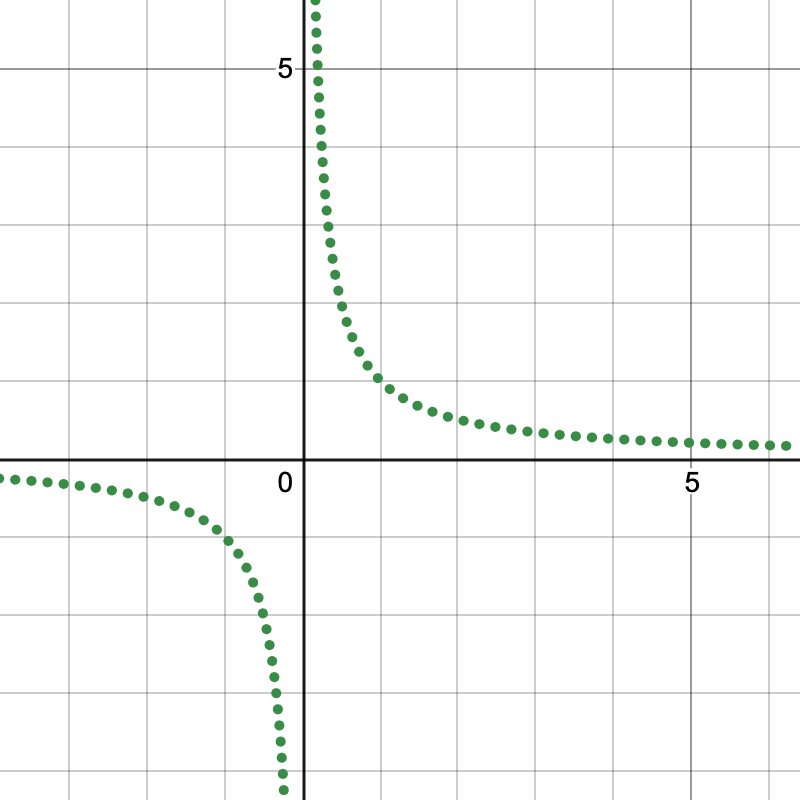
\includegraphics[scale=0.2]{/Users/rudiks/Desktop/Plantilla/images/1/unovern.png}
	\end{center}
$\implies \inf\left(\frac{1}{n}\right)=0$. 
\end{ejemplo}

\begin{ejemplo}
\item $\sup[a,b]=b; \inf[a,b]=a$. 
\item $\sup (a,b)=b; \inf(a,b)=a$. 
\end{ejemplo}

\begin{nota}
	\begin{enumerate}
		\item Si el $\sup A\in A\implies \sup A$ es el máximo de $A$. 
		\item Si el $\inf A\in A\implies \inf A$ es el mínimo de $A$. 
	\end{enumerate}
\end{nota}

\begin{cajita}
	Convenciones: 
	\begin{enumerate}
		\item Si $A$ no está acotada superiormente, entonces escribimos
	$$\sup A=\infty$$
\item Si $A$ no está acotado inferiormente, entonces escribimos 
$$\inf A=-\infty$$	
\item Si $A=\emptyset$ (Recordemos que cada número real es cota superior e inferior de $\emptyset$), se escribe: 

$$\sup \emptyset =-\infty \text{ e } \inf \emptyset = \infty$$
\end{enumerate}
\end{cajita}

\begin{nota}
	En todo caso, se dice que el $\sup A$ e $\inf A$ existen si son un úmero finito. 
\end{nota}

\subsection{Espacios métricos}

\begin{definicion}
	Sea $X$ un conjunto y 
	$$d: X\times X\to \mathbb{R} \ni$$
	$\forall a,b,c\in X$ satisface: 
	\begin{enumerate}
		\item Positividad. $d(a,b)\geq 0$; $d(a,b)=0\iff a=b$. 
		\item Simetría. $d(a,b)=d(b,a)$. 
		\item Desigualdad triiangular. $d(a,b)\leq d(a,c)+d(c,d)$, entonces ($X,d$) es un espacio métrico y $d$ es una métrica sobre $X$ o una distancia sobre $X$. 	\end{enumerate}
\end{definicion}

\begin{prop}[Reordonamiento de la desigualdad triangular]
	Si $(X,d)$ es un espacio métrico y si $a,b,c\in X$, entonces: 
	$$|d(a,b)-d(b,c)|\leq d(a,c).$$
\end{prop}

\begin{ejemplo}
	\begin{enumerate}
		\item Sea $X=\mathbb{R}$ y $d_1:\mathbb{R}\times \mathbb{R}\to \mathbb{R}\ni d_1(a,b)=|a-b|$. $\implies (\mathbb{R},d_1)$ es un espacio métrico. En efecto, sean $a,b,c\in \mathbb{R}$. Entonces: 
		\begin{enumerate}
			\item Pior definición, $d_1(a,b)=|a-b|\geq 0$. 
			\begin{enumerate}
				\item Si $d(a,b)= |a-b|=0\implies a-b=0\implies a=b$. 
				\item Si $a=b\implies d(a,b)=|a-a|=|0|=0$.
			\end{enumerate}
			\item $d(a,b)=|a-b|=|-(a-b)|=|b-a|=d(b,a)$.
			\item $d(a,b)=|a-b|=|(a-c)+(c-d)|\leq |a-c|+|c-b|=d(a,c)+d(c,b)$.
		\end{enumerate}
	\item Cada conjunto admite una métrica. Sea $X\neq \emptyset$, entonces se define la métrica discreta así: $d:X\times X\to \mathbb{R}\ni$ 
	$$d(a,b)=\begin{cases}1, & a\neq b\\ 0, & a=b\end{cases}$$
	$\implies (X,d)$ es espacio métrico.  
	\end{enumerate}
\end{ejemplo}

\begin{ejemplo}[Métrica Euclidiana en $\mathbb{R}^n$]
	Sea $X=\mathbb{R}^n$ y sean: 
	$x=(x_1,\cdots, x_n), y=(y_1,\cdots, y_n)\in \mathbb{R}^n$. Definamos: $d_2:\mathbb{R}^n\times \mathbb{R}^n\to \mathbb{R}\ni$ 
$$d_2(x,y)=\sqrt{\sum_{i=1}^{n}}\left(x_i-y_i\right)^2.$$
$\implies (\mathbb{R}^n, d_2)$ es métrica. 
\end{ejemplo}

\begin{lema}
	Sean $a_1,a_2,\cdots, a_n, b_1,b_2, \cdots, b_n$, números reales cualquiera. Entonces, se cumplen: 
	\begin{enumerate}
		\item Desigualdad de Cauchy-Schwarz
		\begin{align*}
			\left(\sum_{i=1}^{n}a_ib_i\right)^2&\leq \left(\sum_{i=1}^{n}a_i^2\right)\left(\sum_{i=1}^{n}b_i^2\right)\\
			(\overline{a}\cdot \overline{b})&\leq \lVert \overline{a} \rVert\cdot \lVert \overline{b} \rVert
		\end{align*}
	\item Desigualdad de Minkowski 
	$$\left[\sum_{i=1}^n (a_i+b_i)^2\right]^{1/2}\leq \left[\sum_{i=1}^{n}a_i^2\right]+\left[\sum_{i=1}^n b_i^2\right]^{1/2}$$
	\end{enumerate}
\end{lema}

\begin{ejemplo}
	Considere $d_\infty: \mathbb{R}^n\times \mathbb{R}^n\to \mathbb{R}\ni$ 
	$$d_\infty (x,y)=\max\left\{|x_i-y_i|:i=1,\cdots, n\right\}.$$
	$\implies d_\infty$ es una métrica en $\mathbb{R}^n$. 
\end{ejemplo}

\begin{ejemplo}
	$x=(2,3,4)$ y $y=(-1,2,0)$. 
	$$\implies d_\infty(x,y)=\max\left\{|2-(-1)|,|3-2|,|4-0|\right\}=\max\left\{3,1,4\right\}=4.$$
\end{ejemplo}

\begin{ejemplo}
	Sea $B\left([a,b]\right)$ el conjunto de funciones acotadas definidas en $[a,b]$ y de valores reales. También se denota: 
	$$l^{\infty}\left([a,b]\right)=\left\{f:[a,b]\to \mathbb{R}\ni |f(x)|\leq M, M>0\right\}$$.
	$\implies$ Dadas $f,g\in l^{\infty}[a,b]$. 
	
	\begin{center}
		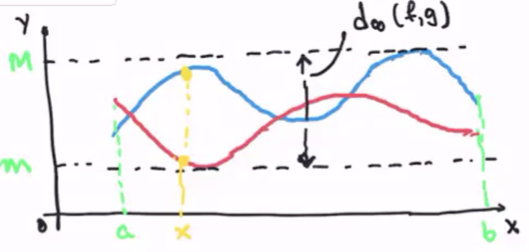
\includegraphics[scale=0.5]{/Users/rudiks/Desktop/Plantilla/images/1/2.png}
	\end{center}
$\implies d_\infty(f,g)=\sup \left\{|f(x)-g(x)|\right\}$, la cual es una métrica en $l^{\infty}[a,b]$ y se llama métrica o distancia del supremo.
\end{ejemplo}

\begin{ejemplo}
	Sea $C[a,b]$ el conjunto de funciones continuas sobre $[a,b]$ con valores reales. Entonces, si $f,g\in C[a,b]$, se tiene la métrica: $$d(f,g)=\int_a^b |f(x)-g(x)|dx$$
	sobre $C[a,b]$. 
\end{ejemplo}

\begin{definicion}
Suponga que $V$ es un espacio vectorail sobre el campo $\mathbb{F}$ ($\mathbb{R}$ o $\mathbb{C}$) y que: 
$$\lVert \cdot \rVert: V\to \mathbb{R}\ni $$
$\forall x,y\in V$ y $\alpha \in\mathbb{F}$ se cumplen: 
\begin{enumerate}
	\item $\lVert x\rVert\geq 0, \lVert x\rVert =0 \iff x=0$. 
	\item $\lVert \alpha x \rVert = |\alpha| \cdot \lVert x \rVert$. 
	\item $\lVert x+y\rVert \leq \lVert x\rVert + \lVert y\rVert$. 
\end{enumerate}
Entonces, $\lVert \cdot \rVert$ es una norma sobre $V$ y decimos que $(V, \lVert\cdot \rVert)$ es un espacio normado.
\end{definicion}

\begin{nota}
	Sea $V$ un espacio vectorial normado. Entonces, considere: 
	$$d:V\times V \to \mathbb{R}\ni$$
	$$d(x,y)=\lVert x-y \rVert.$$
	
	Nótese que: 
	
	\begin{enumerate}
		\item $d(x,y)=\lVert x-y\rVert \geq 0$; 
		\begin{enumerate}
			\item Si $x=y\implies d(x,y)=\lVert x-y\rVert =0$. 
\item Si $d(x,y)=\lVert x-y \rVert =0 \implies x-y=0 \implies x=y$.		
			\end{enumerate}
		
		\item $d(x,y)=\lVert x-y \rVert = \lVert -(y-x)\rVert = |-1|\cdot \lVert y-x\rVert = \lVert y-x\rVert = d(y,x)$. 
		\item $d(x,y)= \lVert x-y\rVert = \lVert (x-z)+(z-y)\rVert \leq \lVert x-<\rVert + \lvert z-y \rVert = d(x,z)+d(z,y)$. $\implies$ $d(x,y)=\lVert x-y\rVert$ es una métrica sobre $V$. Esta es la métrica inducida por la norma.
	\end{enumerate}
\end{nota}